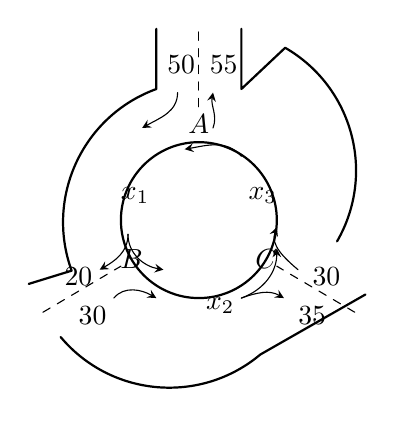
\begin{tikzpicture}[>=stealth, scale=0.9, line cap=round, line join=round]
  % Inner island
  \draw[thick] (0, 0) circle (1.1);

  % Outer roundabout arcs and arms
  % Arm A (top, 90 deg)
  \draw[thick] (-0.6, 2.7) -- (-0.6, 1.85) arc[start angle=110, end angle=200, radius=2.0] -- (-2.4, -0.9);
  \draw[thick] (-1.95, -1.65) arc[start angle=220, end angle=310, radius=2.0] -- (2.35, -1.05);
  \draw[thick] (1.95, -0.3) arc[start angle=330, end angle=420, radius=2.0] -- (0.6, 1.85) -- (0.6, 2.7);

  % Centerlines of branches (dashed)
  \draw[dashed] (0, 1.6) -- (0, 2.7);
  \draw[dashed] (-2.2, -1.3) -- (-1.1, -0.65);
  \draw[dashed] (2.2, -1.3) -- (1.1, -0.65);

  % Branch A flow arrows
  \draw[->] (-0.3, 1.8) to[out=270, in=30] (-0.8, 1.3);
  \draw[->] (0.2, 1.3) to[out=70, in=260] (0.2, 1.8);
  \draw[->] (0.6, 0.9) to[out=130, in=10] (-0.2, 1.0);

  % Branch B flow arrows
  \draw[->] (-1.0, -0.2) to[out=270, in=30] (-1.4, -0.7);
  \draw[->] (-1.0, -0.2) to[out=270, in=170] (-0.5, -0.7);
  \draw[->] (-1.2, -1.1) to[out=50, in=150] (-0.6, -1.1);

  % Branch C flow arrows
  \draw[->] (0.6, -1.1) to[out=20, in=150] (1.2, -1.1);
  \draw[->] (0.6, -1.1) to[out=20, in=270] (1.1, -0.4);
  \draw[->] (1.4, -0.7) to[out=140, in=250] (1.1, -0.1);

  % Numbers
  \node at (-0.25, 2.2) {$50$};
  \node at (0.35, 2.2) {$55$};

  \node at (-1.7, -0.8) {$20$};
  \node at (-1.5, -1.35) {$30$};

  \node at (1.8, -0.8) {$30$};
  \node at (1.6, -1.35) {$35$};

  % Node labels
  \node at (0, 1.35) {$A$};
  \node at (-0.95, -0.55) {$B$};
  \node at (0.95, -0.55) {$C$};

  % Flow variables
  \node at (-0.9, 0.35) {$x_1$};
  \node at (0.3, -1.2) {$x_2$};
  \node at (0.9, 0.35) {$x_3$};
\end{tikzpicture}
